\documentclass[11pt]{article}

\usepackage[spanish]{babel}
\usepackage{translations}
\usepackage[titles]{tocloft}
\usepackage{multicol}
\usepackage{graphicx} % Required for the inclusion of images
\usepackage{amsmath} % Required for some math elements 
\usepackage{hyperref}
\usepackage{amsmath}
\usepackage{listings}
\usepackage{courier}
\usepackage[margin=1in]{geometry}
\usepackage{changepage}
\usepackage{titlesec}
\usepackage{wrapfig}
\usepackage[version=4]{mhchem}
\usepackage{multirow}
\usepackage{siunitx}
\usepackage{ragged2e}
\usepackage{adjustbox}
\usepackage[font=small,labelfont=bf]{caption}
\usepackage[table,xcdraw]{xcolor}
\usepackage{afterpage}
\usepackage{xfrac}
\usepackage{animate}

\definecolor{codegreen}{rgb}{0,0.6,0}
\definecolor{codegray}{rgb}{0.5,0.5,0.5}
\definecolor{codepurple}{rgb}{0.58,0,0.82}
\definecolor{backcolour}{rgb}{0.95,0.95,0.92}

\lstdefinestyle{mystyle}{
    backgroundcolor=\color{backcolour},   
    commentstyle=\color{codegreen},
    keywordstyle=\color{magenta},
    numberstyle=\tiny\color{codegray},
    stringstyle=\color{codepurple},
    basicstyle=\ttfamily\footnotesize,
    breakatwhitespace=false,         
    captionpos=b,                    
    keepspaces=true,                 
    numbers=left,                    
    numbersep=5pt,                  
    showspaces=false,                
    showstringspaces=false,
    showtabs=false,                  
    tabsize=2
}
\lstset{language=Python, 
        basicstyle=\ttfamily\small, 
        keywordstyle=\color{keywords},
        commentstyle=\color{comments},
        stringstyle=\color{red},
        showstringspaces=false,
        identifierstyle=\color{codepurple},
        keywords=[2]{pow},
        keywordstyle=[2]{\color{orange}},
}

\lstset{style=mystyle}
\setlength\parindent{0pt}
\renewcommand{\labelenumi}{\alph{enumi}.}

\setlength\parindent{0pt} % Removes all indentation from paragraphs

\renewcommand{\labelenumi}{\alph{enumi}.} % Make numbering in the enumerate environment by letter rather than number (e.g. section 6)
   
\newcommand{\titulo}{Campos Magnéticos\\\ \\(Práctica 2)}
\newcommand{\nombreestudiante}{Víctor Mira Ramírez\\ Lucas Peydró Ferrando}
\newcommand{\nombredirector}{María Reyes Calvo Urbina}
\newcommand{\fecha}{\date{Junio 2023}}  % Definir solo el año de presentación

\pagebreak

\renewcommand{\listtablename}{Índice de tablas} 
\renewcommand{\tablename}{Tabla} 
\renewcommand\cftsecdotsep{\cftdotsep}

\setlength{\cftbeforesecskip}{0.5ex}
\renewcommand{\cftsecfont}{%
  \fontsize{11}{13}\usefont{OT1}{phv}{bc}{n}\selectfont
}
\makeatletter
\renewcommand{\@pnumwidth}{1.75em}
\renewcommand{\@tocrmarg}{2.75em}
\makeatother

\begin{document}

\begin{titlepage}
	\centering
	
\includegraphics[width=65mm]{fotos/logoUA.png}\par
	\vspace{1cm}
	{\huge\bfseries \vspace{15mm} \titulo \par}
	\vfill
	{\large 
	\vfill
	Estudiantes:\par\vspace{2mm}
	\nombreestudiante\par
	\vfill
	Profesora:\par\vspace{2mm}
    \nombredirector
    \vfill
    Universidad de Alacant\par
    Facultad de Ciencias: Departamento de Física Aplicada\par
    Electromagnetismo 1\par
	\fecha\par}
\end{titlepage}

\pagebreak

\begin{abstract}\label{sec:abstract}
    \noindent Esta práctica tiene como objetivo el cálculo numérico y representación visual del campo magnético generado por una espira por la que circula una corriente eléctrica, un momento dipolar magnético y una distribución de momentos magnéticos.
\end{abstract}

\vspace{0.3cm}
\tableofcontents
\newpage

\vspace{-0.2cm}
\section{Marco teórico}
    \vspace{-0.15cm}
    \subsection{Campo Magnético}
        \noindent Un campo magnético es un concepto matématico que utlizamos para la comprensión de los comportamientos magnéticos generados por un imán, una carga en movimiento o una corriente eléctrica. Una de las características fundamentales del campo magnético es que poseen dos polos (dipolares), polo Norte y polo Sur, por lo tanto sus líneas de campo serán líneas cerradas (salen del polo norte y llegan al polo sur). Durante la práctica representaremos estas líneas de campo, con flechas que nos indicaran la dirección deel campo y el color nos indicará la intensidad de este.
        \vspace{5mm}
        \newline Profundicemos ahora en las fuentes de campo magnético que vamos a estudiar para esta práctica, las corrientes eléctricas y los dipolos magnéticos.
        \vspace{-0.2cm}        
        \subsection{Corriente eléctrica}
        Una corriente eléctrica es un conjunto de cargas eléctricas desplazándose por un material conductor. Por lo tanto, al ser cargas eléctricas en movimiento, estas generarán un campo magnético. El sentido y dirección del campo magnético viene determinado por la regla de la mano derecha: 
        
        \begin{wrapfigure}[6]{r}{0.18\textwidth}
            \vspace{-0.44cm}
            \centering
            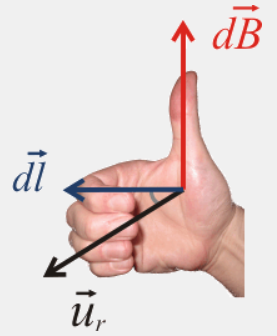
\includegraphics[width=0.14\textwidth]{Captura.PNG}
        \end{wrapfigure}

        \vspace{0.4cm}La forma más habitual de generar un campo magnético es mediante corrientes que circulan por cicuitos filiformes (o cerrados), la contribución de un elemento infinitesimal de longitud dl del circuito recorrido por una corriente I crea una contribución elemental de campo magnético, dB, en el punto situado en la posición que apunta el vector r a una distancia r respecto de d l, quien apunta en la dirección de la corriente I:

        \begin{wrapfigure}[6]{l}{0.2\textwidth}
            \vspace{-0.44cm}
            \centering
            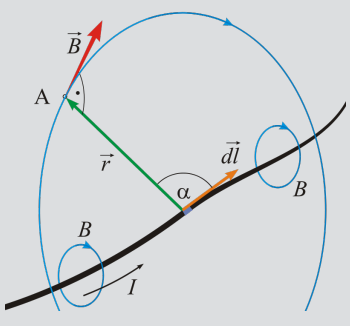
\includegraphics[width=0.2\textwidth]{Captura2.PNG}
        \end{wrapfigure}

        \vspace{0.4cm}Para poder describir el campo magnético empleamos la ley de Biot y Savart (\ref{eq:biotsavart}), que nos proporciona una ecuación que relaciona el campo magnético a la magnitud, la dirección, longitud y proximidad de una corriente eléctrica.

        \begin{equation}
            \centering
                d\vec{B}=\frac{\mu _{0}}{4\pi}\frac{Id\vec{l}\times\hat{r}}{r^{2}}
            \label{eq:biotsavart}
        \end{equation}

        \vspace{0.1cm}
        \subsection{Dipolo magnético}
        Un dipolo magnético es, en cierta manera, una aproximación al campo que genera un circuito cuando la distancia al circuito es mucho mayor que las dimensiones del mismo. 
        \vspace{5mm}
        \newline Los dipolos se caracterizan por su momento dipolar, una magnitud vectorial. Estudianto este fenómeno para un circuito cerrado C, con una corriente I, el momento dipolar lo obtenemos de la siguiente forma:

        \vspace{-0.25cm}
        \begin{equation}
            \centering
                \vec{m}=\frac{1}{2}I\oint_{C}\vec{r}\times d\vec{r}
            \label{eq:dipolo}
        \end{equation}

        \vspace{0.4cm}Una vez definido el momento diporlar, podemos calcular el campo magnético generado por un dipolo de la siguiente forma:

        \vspace{-0.15cm}
        \begin{equation}
            \centering
                \vec{B}(\vec{r})=\vec{\nabla} \times \vec{A}=\frac{\mu_{0}}{4\pi}\left ( \frac{3\vec{r}(\vec{m}\cdot \vec{r})}{r^{5}}-\frac{\vec{m}}{r^{3}} \right )
            \label{eq:campdipolo}
        \end{equation}

\clearpage
\section{Campo magnético debido a una espira}

\vspace{5mm} Mediante un programa desarrollado en python, calcularemos el campo magnético a partir de la ley de Biot-Savart en el punto x,y,z debido a una espira circular de corriente I y de radio R centrada en el origen de coordenadas y situada en el plano z=0. 

\vspace{5mm} Representaremos el campo magnético generado en el plano z=0 para diferentes radios, R=0.5 y R=0.05. Utilizando tanto una representación vectorial como una representación gráfica.

        \begin{figure}[h]
            \centering
            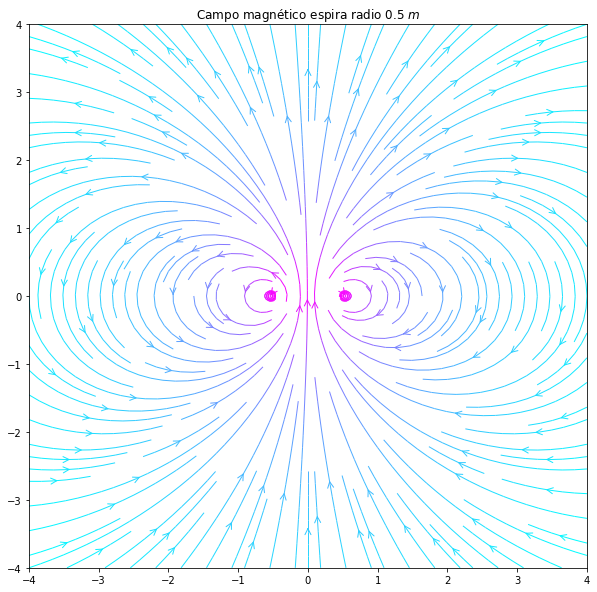
\includegraphics[width=0.35\textwidth]{Mag espira.png}
            \hspace{1cm}
            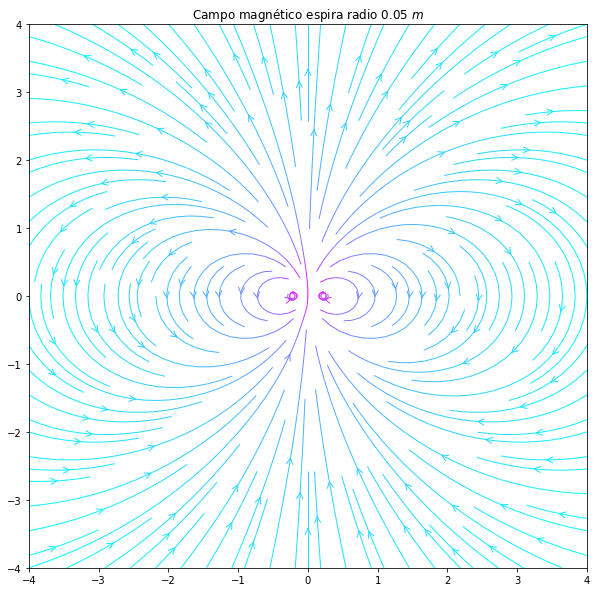
\includegraphics[width=0.35\textwidth]{mag 0.05 espira.png}
            \caption{Campo magnético generado por una espira de radio 0.5m (izq.) y 0.05m (dcha.)}
        \end{figure}


        \begin{figure}[h]
            \centering
            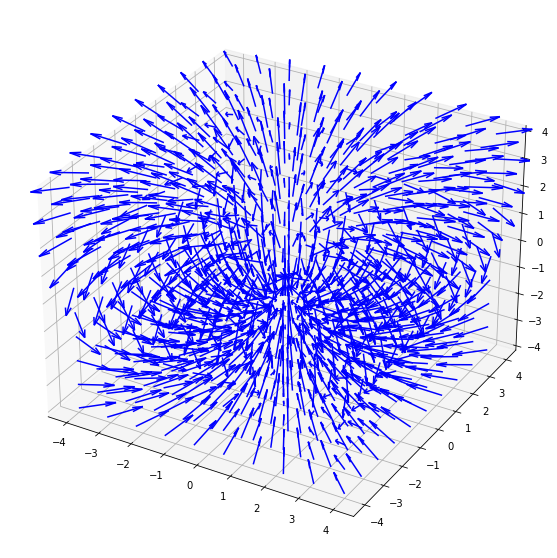
\includegraphics[width=0.35\textwidth]{Mag 3d.png}
            \caption{Representacion 3D del campo magnético de una espira de radio 0.5m}
            \label{fig:my_label}
        \end{figure}

\vspace{5mm} Las figuras anteriores representan el campo magnético generado por una espira por la cual circula una corriente de 1A. El campo magnético que observamos es cerrado (líneas de campo que empiezan y acaban en el mismo lugar, que nunca se llegan a cortar entre ellas), también por los diferentes colores que tiene la figura podemos observar donde este es más intenso. Se observa que la espira de radio 0.5m tiene una mayor intensidad en comparación con la espira de 0.05m. En ambos casos vemos como el campo magnético se reduce con la distancia.
\clearpage
        \begin{figure}[h]
            \centering
            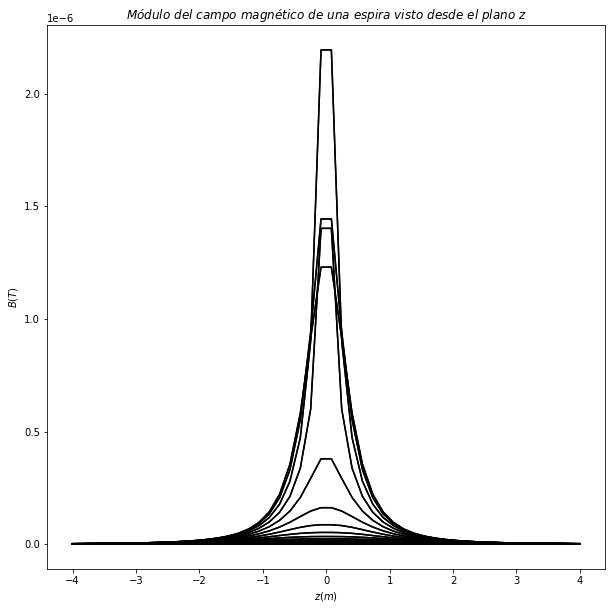
\includegraphics[width=0.35\textwidth]{Mag z.png}
            \hspace{1cm}
            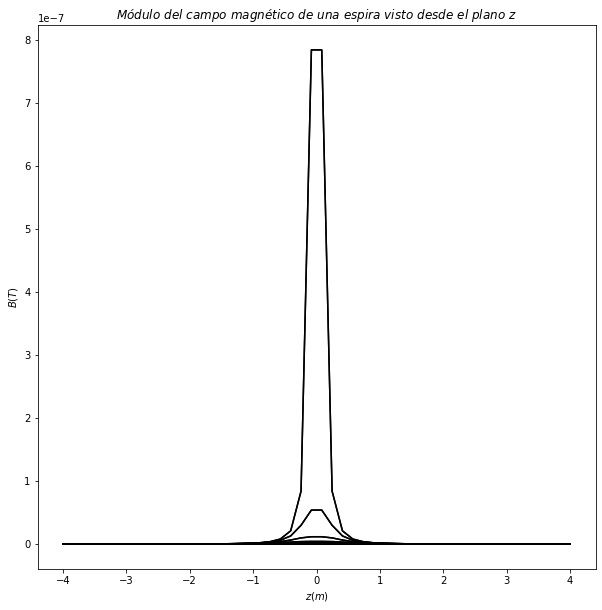
\includegraphics[width=0.35\textwidth]{Mag 0.05 z.png}
            \caption{Perfiles del campo magnético en la direccion z de una espira de radio 0.5m (izq.) y 0.05m (dcha.)}
        \end{figure}

\vspace{5mm} En estas dos últimas figuras podemos apreciar más visiblemente como decae el campo magnético con respecto a la distancia. A su vez, obsevamos como el campo magnético para la espira de radio 0.05m es notablemente menor a la del radio de 0.5m.

\section{Campo magnético debido a un momento dipolar magnético}

\vspace{5mm} Para este apartado hemos creado una función que calcula el campo magnético en el punto x,y,z debido a un momento dipolar magnético m=(mx,mymz) situado en un punto arbitrario del espacio.

\begin{figure}[h]
    \centering
    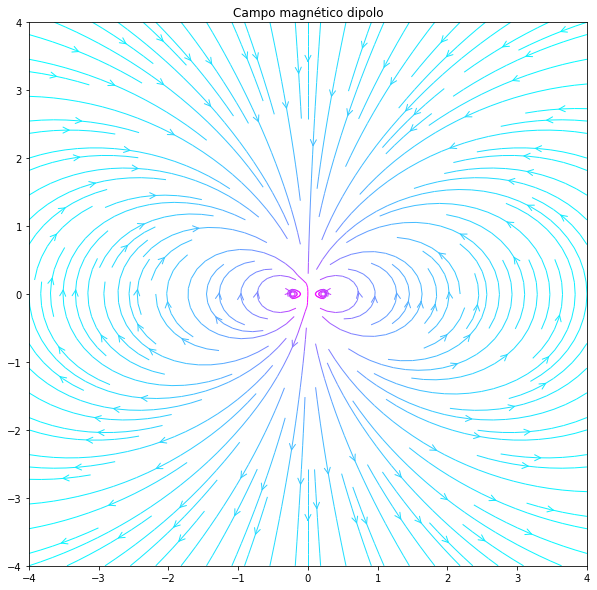
\includegraphics[width=0.35\textwidth]{Mag 0.05 dipolo.png}
    \hspace{1cm}
    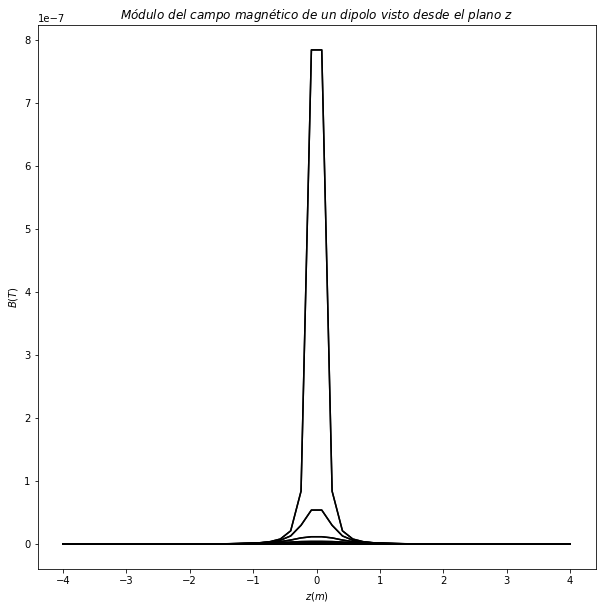
\includegraphics[width=0.342\textwidth]{Mag 0.05 dipolo z.png}
    \caption{Lineas de campo y perfil del campo magnético de un momento dipolar magnético}
\end{figure}

\vspace{5mm} Para este caso podemos sacar las mismas conclusiones que en los apartados anteriores. Ya que las representaciones obtenidas son muy similares a las obtenidas en el apartado de la espira de corriente mediante la ley de Biot-Savart.

\vspace{5mm}
\section{Campo magnético causado por una distribución reticular de momentos magnéticos}
Vamos a calcular el campo magnético de momentos magnéticos, esta vez considerando una distribución reticular. Sabemos que al realizar distribuciones de varios momentos magnéticos el campo total no será más que la superposición de los momentos individuales. 

\vspace{0.4cm}El campo final es la suma del campo generado por cada momento individualmente.

\begin{figure}[h]
    \vspace{-0.4cm}
    \centering
    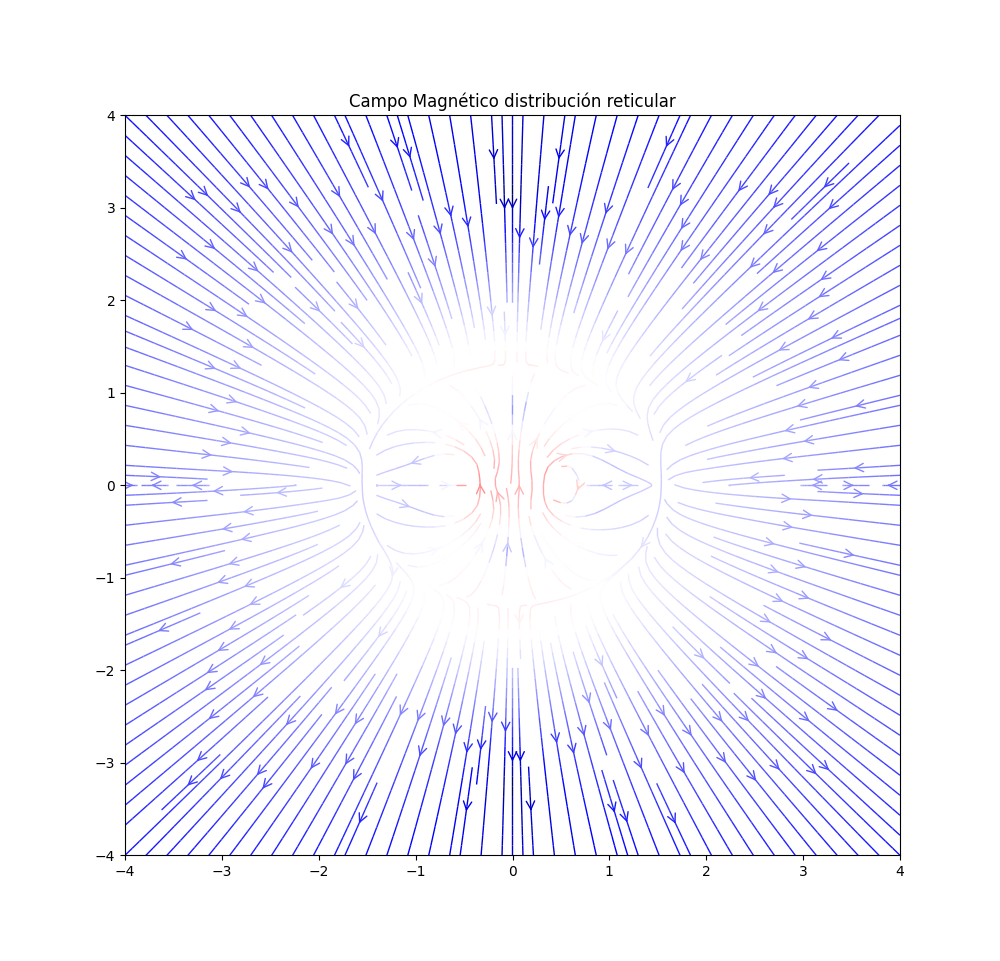
\includegraphics[width=0.6\textwidth]{reticular.png}
    \caption{Campo magnético generado por una distribución reticular de momentos magnéticos}
\end{figure}

Destacar como en la zona interior a la distribución las líneas de campo no son paralelas ya que encontramos bucles alrededor de los distintos momentos y no es hasta que nos alejamos lo suficiente de ellos que dejamos de apreciar a cada uno individualmente y empezamos a ver un paralelismo en las líneas de campo que nos indica que estamos en la zona donde el campo es la suma de todos ellos.\vspace{0.4cm}

Como el mapa de color nos muestra, dentro de la distribución el campo se anula casi en su totalidad ya los campos de los momentos se van cancelando entre sí.

\section{Anexos}
\subsubsection*{Código de python que genera las gráficas:}
\href{https://github.com/vmr48-ua/extras/blob/main/ELEC1-P2.py}{ELEC1-P2.py}
\subsubsection*{Código de LaTeX que genera este documento:}
\href{https://www.overleaf.com/read/xmcwycdmwcny}{ELEC2-Practica2:Campos-Magneticos.tex}
\end{document} 